\begin{table*}[t]
\small
\setlength{\tabcolsep}{2.2pt}{
\begin{tabular}{C{2.0cm}C{3.0cm}|C{2.5cm}C{2.5cm}C{1.5cm}C{1.8cm}C{3.2cm}}
\toprule
     Datasets & Sources & Train (all-normal) & Train (with labels) &  Test& Sample size & Annotation Level \\
    \hline
    BrainMRI & BraTS2021~\cite{baid2021rsna,bakas2017advancing,menze2014multimodal}& 7,500 & 83 & 3,715  &240*240  & Segmentation mask   \\
    LiverCT & BTCV\cite{landman2015miccai} + LiTs~\cite{bilic2023liver} & 1,452 & 166 &1,493  & 512*512 & Segmentation mask  \\
    RESC & RESC~\cite{hu2019automated}& 4,297 & 115 & 1,805  & 512*1,024 & Segmentation mask  \\
    OCT17 & OCT2017~\cite{kermany2018identifying}& 26,315 & 32 &968 & 512*496 & Image label \\
    ChestXray & RSNA~\cite{wang2017chestx}&8,000& 1,490 &17,194 & 1,024*1,024 & Image label    \\
    HIS & Camelyon16~\cite{bejnordi2017diagnostic}&5,088&  236  &2,000 &  256*256 & Image label \\
    \bottomrule
    \end{tabular}
    }
    \caption{Summary of datasets from different medical modalities.}
\label{tal:dataset}
\end{table*}

\begin{figure*}
\noindent\begin{minipage}[t]{0.32\linewidth}
(a) \emph{State}-level (-:normal, +:abnormal)

{\tt \small
\begin{itemize}
    \item[-] c := "[o]"
    \item[-] c := "flawless [o]"
    \item[-] c := "perfect [o]"
    \item[-] c := "unblemished [o]"
    \item[-] c := "[o] without flaw"
    \item[-] c := "[o] without defect"
    \item[-] c := "[o] without damage"
    \item[+] c := "damaged [o]"
    \item[+] c := "[o] with flaw"
    \item[+] c := "[o] with defect"
    \item[+] c := "[o] with damage"
\end{itemize}
}
\end{minipage}
\hfill
\begin{minipage}[t]{0.38\linewidth}
(b) \emph{Template}-level

{\tt \small
\begin{itemize}
\item "a photo of a/the/one [c]."
\item "a photo of a/the cool [c]."
\item "a photo of a/the small [c]."
\item "a photo of a/the large [c]."
\item "a bright photo of a/the [c]." 
\item "a dark photo of a/the [c]."
\item "a blurry photo of a/the [c]."
\item "a bad photo of a/the [c]."
\item "a good photo of a/the [c]."
\item "a cropped photo of a/the [c]."
\item "a close-up photo of a/the [c]."
\end{itemize}
}
\end{minipage}
\begin{minipage}[t]{0.29\linewidth}
{\tt \small
\begin{itemize}
\item {\rm (cont'd)} "a photo of my [c]."
\item "a low resolution photo of a/the [c]."
\item "a black and white photo of a/the [c]."
\item "a jpeg corrupted photo of a/the [c]."
\item "there is a/the [c] in the scene."
\item "this is a/the/one [c] in the scene."
\end{itemize}
}
\end{minipage}
\caption{Lists of state and template level prompts employed in this paper to construct text features.}
\label{fig:comp_prompt}
\vspace{10pt}
\end{figure*}

\begin{table*}[h]
\centering
\caption{Comparisons with state-of-the-art \textbf{few-shot} anomaly detection methods with $K=2,4,8,16$. The AUCs (in \%) for anomaly classification (AC) and anomaly segmentation (AS) are reported. The best result is in bold, and the second-best result is underlined.}
\label{tal:suppfew}
\small
\setlength{\tabcolsep}{2.2pt}{
\begin{tabular}{C{2.0cm}C{2.2cm}C{1.8cm}|C{1.1cm}C{1.2cm}C{1.2cm}|C{1.0cm}C{1.0cm}C{1.0cm}C{1.0cm}C{1.0cm}C{1.0cm}}
\toprule
\multirow{2}{*}{Shot Number} & \multirow{2}{*}{Method} & \multirow{2}{*}{Source} & HIS & ChestXray & OCT17 & \multicolumn{2}{c}{BrainMRI} & \multicolumn{2}{c}{LiverCT} & \multicolumn{2}{c}{RESC}\\
\cmidrule(lr){4-12} 
& & & AC & AC & AC & AC & AS & AC & AS & AC & AS\\
\cmidrule(lr){1-12} 
& DRA~\cite{DRA} & CVPR 2022 & \underline{72.91} & \underline{72.22} & \underline{98.08} & 71.78 & 72.09 & 57.17 & 63.13 & 85.69 & 65.59 \\
& BGAD~\cite{BGAD} & CVPR 2023 & - & - & - & \underline{78.70}  & 92.42 & \underline{72.27} & \textbf{98.71} & 83.58 & 92.10 \\
& APRIL-GAN~\cite{chen2023zero} & arXiv 2023   & 69.57 & 69.84 & \textbf{99.21} & 78.45 & \underline{94.02} & 57.80 & 95.87 & \underline{89.44} & \underline{96.39} \\
\multirow{-4}{*}{2-shot} & MFA & ours & \textbf{82.61} & \textbf{81.32} & 97.98 & \textbf{92.72} & \textbf{96.55} & \textbf{81.08} & \underline{96.57} & \textbf{91.36} & \textbf{98.11} \\
\cmidrule(lr){1-12} 
& DRA~\cite{DRA} & CVPR 2022 & 68.73 & 75.81 & 99.06 & 80.62 & 74.77 & 59.64 & 71.79 & 90.90 & 77.28 \\
& BGAD~\cite{BGAD} & CVPR 2023 & - & - & - & 83.56 & 92.68 & \underline{72.48} & \underline{98.88} & 86.22 & 93.84 \\
& APRIL-GAN~\cite{chen2023zero} & arXiv 2023   & \underline{76.11} & \underline{77.43} & \textbf{99.41} & \underline{89.18} & \underline{94.67} & 53.05 & 96.24 & \underline{94.70}  & \underline{97.98} \\
\multirow{-4}{*}{4-shot} & MFA & ours & \textbf{82.71} & \textbf{81.95} & \underline{99.38} & \textbf{92.44} & \textbf{97.30}  & \textbf{81.18} & \textbf{99.73} & \textbf{96.18} & \textbf{98.97} \\
\cmidrule(lr){1-12} 
& DRA~\cite{DRA} & CVPR 2022 & 74.33 & \underline{82.70}  & 99.13 & 85.94 & 75.32 & 72.53 & 81.78 & \underline{93.06} & 83.07 \\
& BGAD~\cite{BGAD} & CVPR 2023 & - & - & - & 88.01 & 94.32 & \underline{74.60} & \underline{99.00} & 89.96 & 96.06\\
& APRIL-GAN~\cite{chen2023zero} & arXiv 2023   & \underline{81.70}  & 73.69 & \textbf{99.75} & \underline{88.41} & \underline{95.50}  & 62.38 & 97.56 & 91.36 & \underline{97.36} \\
\multirow{-4}{*}{8-shot} & MFA & ours & \textbf{85.10}  & \textbf{83.89} & \underline{99.64} & \textbf{92.61} & \textbf{97.21} & \textbf{85.90} & \textbf{99.79} & \textbf{96.57} & \textbf{99.00} \\
\cmidrule(lr){1-12} 
& DRA~\cite{DRA} & CVPR 2022 & 79.16 & \underline{85.01} & \underline{99.87} & 82.99 & 80.45 & 80.89 & 93.00 & 94.88 & 84.01 \\
& BGAD~\cite{BGAD} & CVPR 2023 & - & - & - & 88.05 & 95.29 & 78.79 & 99.25 & 91.29 & 97.07 \\
& APRIL-GAN~\cite{chen2023zero} & arXiv 2023   & \underline{81.16} & 78.62 & \textbf{99.93} & \underline{94.03} & \underline{96.17} & \underline{82.94} & \underline{99.64} & \underline{95.96} & \underline{98.47} \\
\multirow{-4}{*}{16-shot}  & MFA & ours & \textbf{82.62} & \textbf{85.72} & 99.66 & \textbf{94.40}  & \textbf{97.70}  & \textbf{83.85} & \textbf{99.73} & \textbf{97.25} & \textbf{99.07}\\
\bottomrule
\end{tabular}
}
\end{table*}

\newpage
\clearpage
\appendix
\section{Medical Anomaly Detection Benchmark}\label{sec:ap_dataset}

The details of the medical anomaly detection (AD) benchmark are concisely summarized in Table~\ref{tal:dataset}. For the few-shot AD scenario, we select a random subset of labeled training samples, with $K\in \{2,4,8,16\}$, from the labeled training set (designated as ``Train (with labels)'' in Table~\ref{tal:dataset}). These samples are employed in various competing baselines, including CLIP~\cite{openclip}, WinCLIP~\cite{winclip}, DRA~\cite{DRA}, BGAD~\cite{BGAD}, and April-GAN~\cite{chen2023zero}. Furthermore, consistent with the original methodologies that require training on a substantial amount of normal data, such as CFlowAD~\cite{gudovskiy2022cflow}, RD4AD~\cite{deng2022anomaly}, PatchCore~\cite{patchcore}, and MKD~\cite{MKD}, we employ a dataset exclusively comprising normal images. This dataset is referred to as ``Train (all-normal)'' for training purposes. It is important to highlight that this ``all-normal'' training set encompasses considerably more data compared to the limited data used in the few-shot scenario.
Below are detailed descriptions of datasets used in medical AD benchmark:

\begin{table*}[h!]
\centering
\caption{Ablation study of multi-level features \textbf{without multi-level training}. The AUCs (in \%) for classification (AC) and segmentation (AS) under the few-shot setting (k=4) are reported. The best result is in bold, and the second-best result is underlined.}
\label{tal:supplayer_2}
\small
\setlength{\tabcolsep}{2.5pt}{
\begin{tabular}{C{2.5cm}|C{1.4cm}C{1.4cm}C{1.4cm}|C{1.4cm}C{1.4cm}C{1.4cm}C{1.4cm}C{1.4cm}C{1.4cm}}
\toprule
\multirow{2}{*}{Layers} & HIS & ChestXray & OCT17 & \multicolumn{2}{c}{BrainMRI} & \multicolumn{2}{c}{LiverCT} & \multicolumn{2}{c}{RESC}\\
\cmidrule(lr){2-10} 
& AC & AC & AC & AC & AS & AC & AS & AC & AS\\
\cmidrule(lr){1-10} 
Layer 1 & 74.54 & 78.69 & 97.75 & 87.84 & 97.05 & 58.15 & 98.47 & 88.76 & 97.58\\
Layer 2 & \underline{81.36} & \underline{81.09} & \textbf{99.84} & \underline{90.81} & \textbf{97.34} & \textbf{85.36} & \underline{99.58} & \underline{94.54} & \underline{98.81}\\
Layer 3 & 69.00 & 79.75 & 98.68 & 83.01 & 94.34 & 63.78 & 95.35 & 93.29 & 98.40\\
Layer 4 & 71.02 & 72.84 & 99.37 & 86.92 & 95.42 & 76.09 & 97.92 & 93.72 & 98.23\\
\cmidrule(lr){1-10} 
Ensemble & \textbf{82.71} & \textbf{81.95} & \underline{99.38} & \textbf{92.44} & \underline{97.30} & \underline{81.18} & \textbf{99.73} & \textbf{96.18} & \textbf{98.97}\\
\bottomrule
\end{tabular}
}
\end{table*}

\begin{table*}[h!]
\centering
\caption{Ablation study of multi-level features \textbf{with multi-level training}. The AUCs (in \%) for classification (AC) and segmentation (AS) under the few-shot setting (k=4) are reported. The best result is in bold, and the second-best result is underlined.}
\label{tal:supplayer}
\small
\setlength{\tabcolsep}{2.5pt}{
\begin{tabular}{C{2.5cm}|C{1.4cm}C{1.4cm}C{1.4cm}|C{1.4cm}C{1.4cm}C{1.4cm}C{1.4cm}C{1.4cm}C{1.4cm}}
\toprule
\multirow{2}{*}{Layers} & HIS & ChestXray & OCT17 & \multicolumn{2}{c}{BrainMRI} & \multicolumn{2}{c}{LiverCT} & \multicolumn{2}{c}{RESC}\\
\cmidrule(lr){2-10} 
& AC & AC & AC & AC & AS & AC & AS & AC & AS\\
\cmidrule(lr){1-10} 
Layer 1 & 71.19 & 78.80 & 94.82 & 87.47 & 97.13 & 80.04 & \underline{99.67} & 88.03 & 97.15\\
Layer 2 & 80.88 & \textbf{83.56} & \textbf{99.49} & 92.41 & \textbf{97.35} & 80.98 & 99.61 & \underline{95.73} & \underline{98.90}\\
Layer 3 & \underline{82.35} & 58.32 & 96.96 & \textbf{93.01} & 97.14 & 81.10 & 99.59 & 94.18 & \underline{98.90}\\
Layer 4 & 81.43 & 64.58 & 95.36 & \underline{92.86} & 94.43 & \textbf{81.32} & 99.59 & 92.17 & 98.31\\
\cmidrule(lr){1-10} 
Ensemble & \textbf{82.71} & \underline{81.95} & \underline{99.38} & 92.44 & \underline{97.30} & \underline{81.18} & \textbf{99.73} & \textbf{96.18} & \textbf{98.97}\\
\bottomrule
\end{tabular}
}
\end{table*}

\begin{table*}[t]
    \centering
    \caption{Comparisons with state-of-the-art methods on in-domain dataset MVTec AD. The AUCs (in \%) for classification (AC) and segmentation (AS) under the few-shot setting (k=4) are reported.}
    \label{tal:s7_in2}
    \small
    \setlength{\tabcolsep}{2.2pt}{
    \begin{tabular}{C{2.3cm}C{1.4cm}C{1.4cm}C{1.4cm}C{1.4cm}C{1.4cm}C{1.4cm}C{1.4cm}C{1.4cm}}
    \toprule
\multirow{2}{*}{\begin{tabular}{c} 
Category (k=4)
\end{tabular}} & \multicolumn{2}{c}{RegAD} & \multicolumn{2}{c}{ WinCLIP } & \multicolumn{2}{c}{ April-GAN } & \multicolumn{2}{c}{ MVFA } \\
\cmidrule(lr){2-9}  
& AC & AS & AC & AS & AC & AS & AC & AS \\
\cmidrule(lr){1-9} 
bottle & 99.3 & 98.5 & 99.3 & 97.8 & 94.2 & 97.2 & 99.8 & 98.7 \\
cable & 82.9 & 95.5 & 90.9 & 94.9 & 76.7 & 91.8 & 88.0 & 87.3 \\
capsule & 77.3 & 98.3 & 82.3 & 96.2 & 93.5 & 97.5 & 93.9 & 96.0 \\
carpet & 97.9 & 98.9 & 100 & 99.3 & 99.9 & 98.7 & 100 & 99.4 \\
grid & 87.0 & 85.7 & 99.6 & 98.0 & 99.2 & 97.6 & 100 & 96.9 \\
hazelnut & 95.9 & 98.4 & 98.4 & 98.8 & 98.8 & 97.7 & 99.7 & 98.1 \\
leather & 99.9 & 99.0 & 100 & 99.9 & 100 & 99.5 & 99.9 & 99.4 \\
metal nut & 94.3 & 96.5 & 99.5 & 92.9 & 91.0 & 93.1 & 99.4 & 99.3 \\
pill & 74.0 & 97.4 & 92.8 & 97.1 & 84.1 & 95.5 & 95.1 & 96.8 \\
screw & 59.3 & 96.0 & 87.9 & 96.0 & 83.7 & 98.5 & 88.3 & 98.5 \\
tile & 98.2 & 92.6 & 99.9 & 96.6 & 99.1 & 96.0 & 99.7 & 98.7 \\
toothbrush & 91.1 & 98.5 & 96.7 & 98.4 & 93.2 & 98.8 & 95.8 & 98.8 \\
transistor & 85.5 & 93.5 & 85.7 & 88.5 & 84.1 & 83.7 & 84.3 & 80.9 \\
wood & 98.9 & 96.3 & 99.8 & 95.4 & 98.7 & 96.2 & 99.7 & 97.2 \\
zipper & 95.8 & 98.6 & 94.5 & 94.2 & 95.4 & 96.6 & 99.3 & 98.9 \\
\hline average & 89.2 & 96.2 & 95.2 & \textbf{96.3} & 92.8 & 95.9 & \textbf{96.2} & \textbf{96.3} \\
\bottomrule
\end{tabular}}
\end{table*}

\begin{figure*}[h!]
    \centering    
    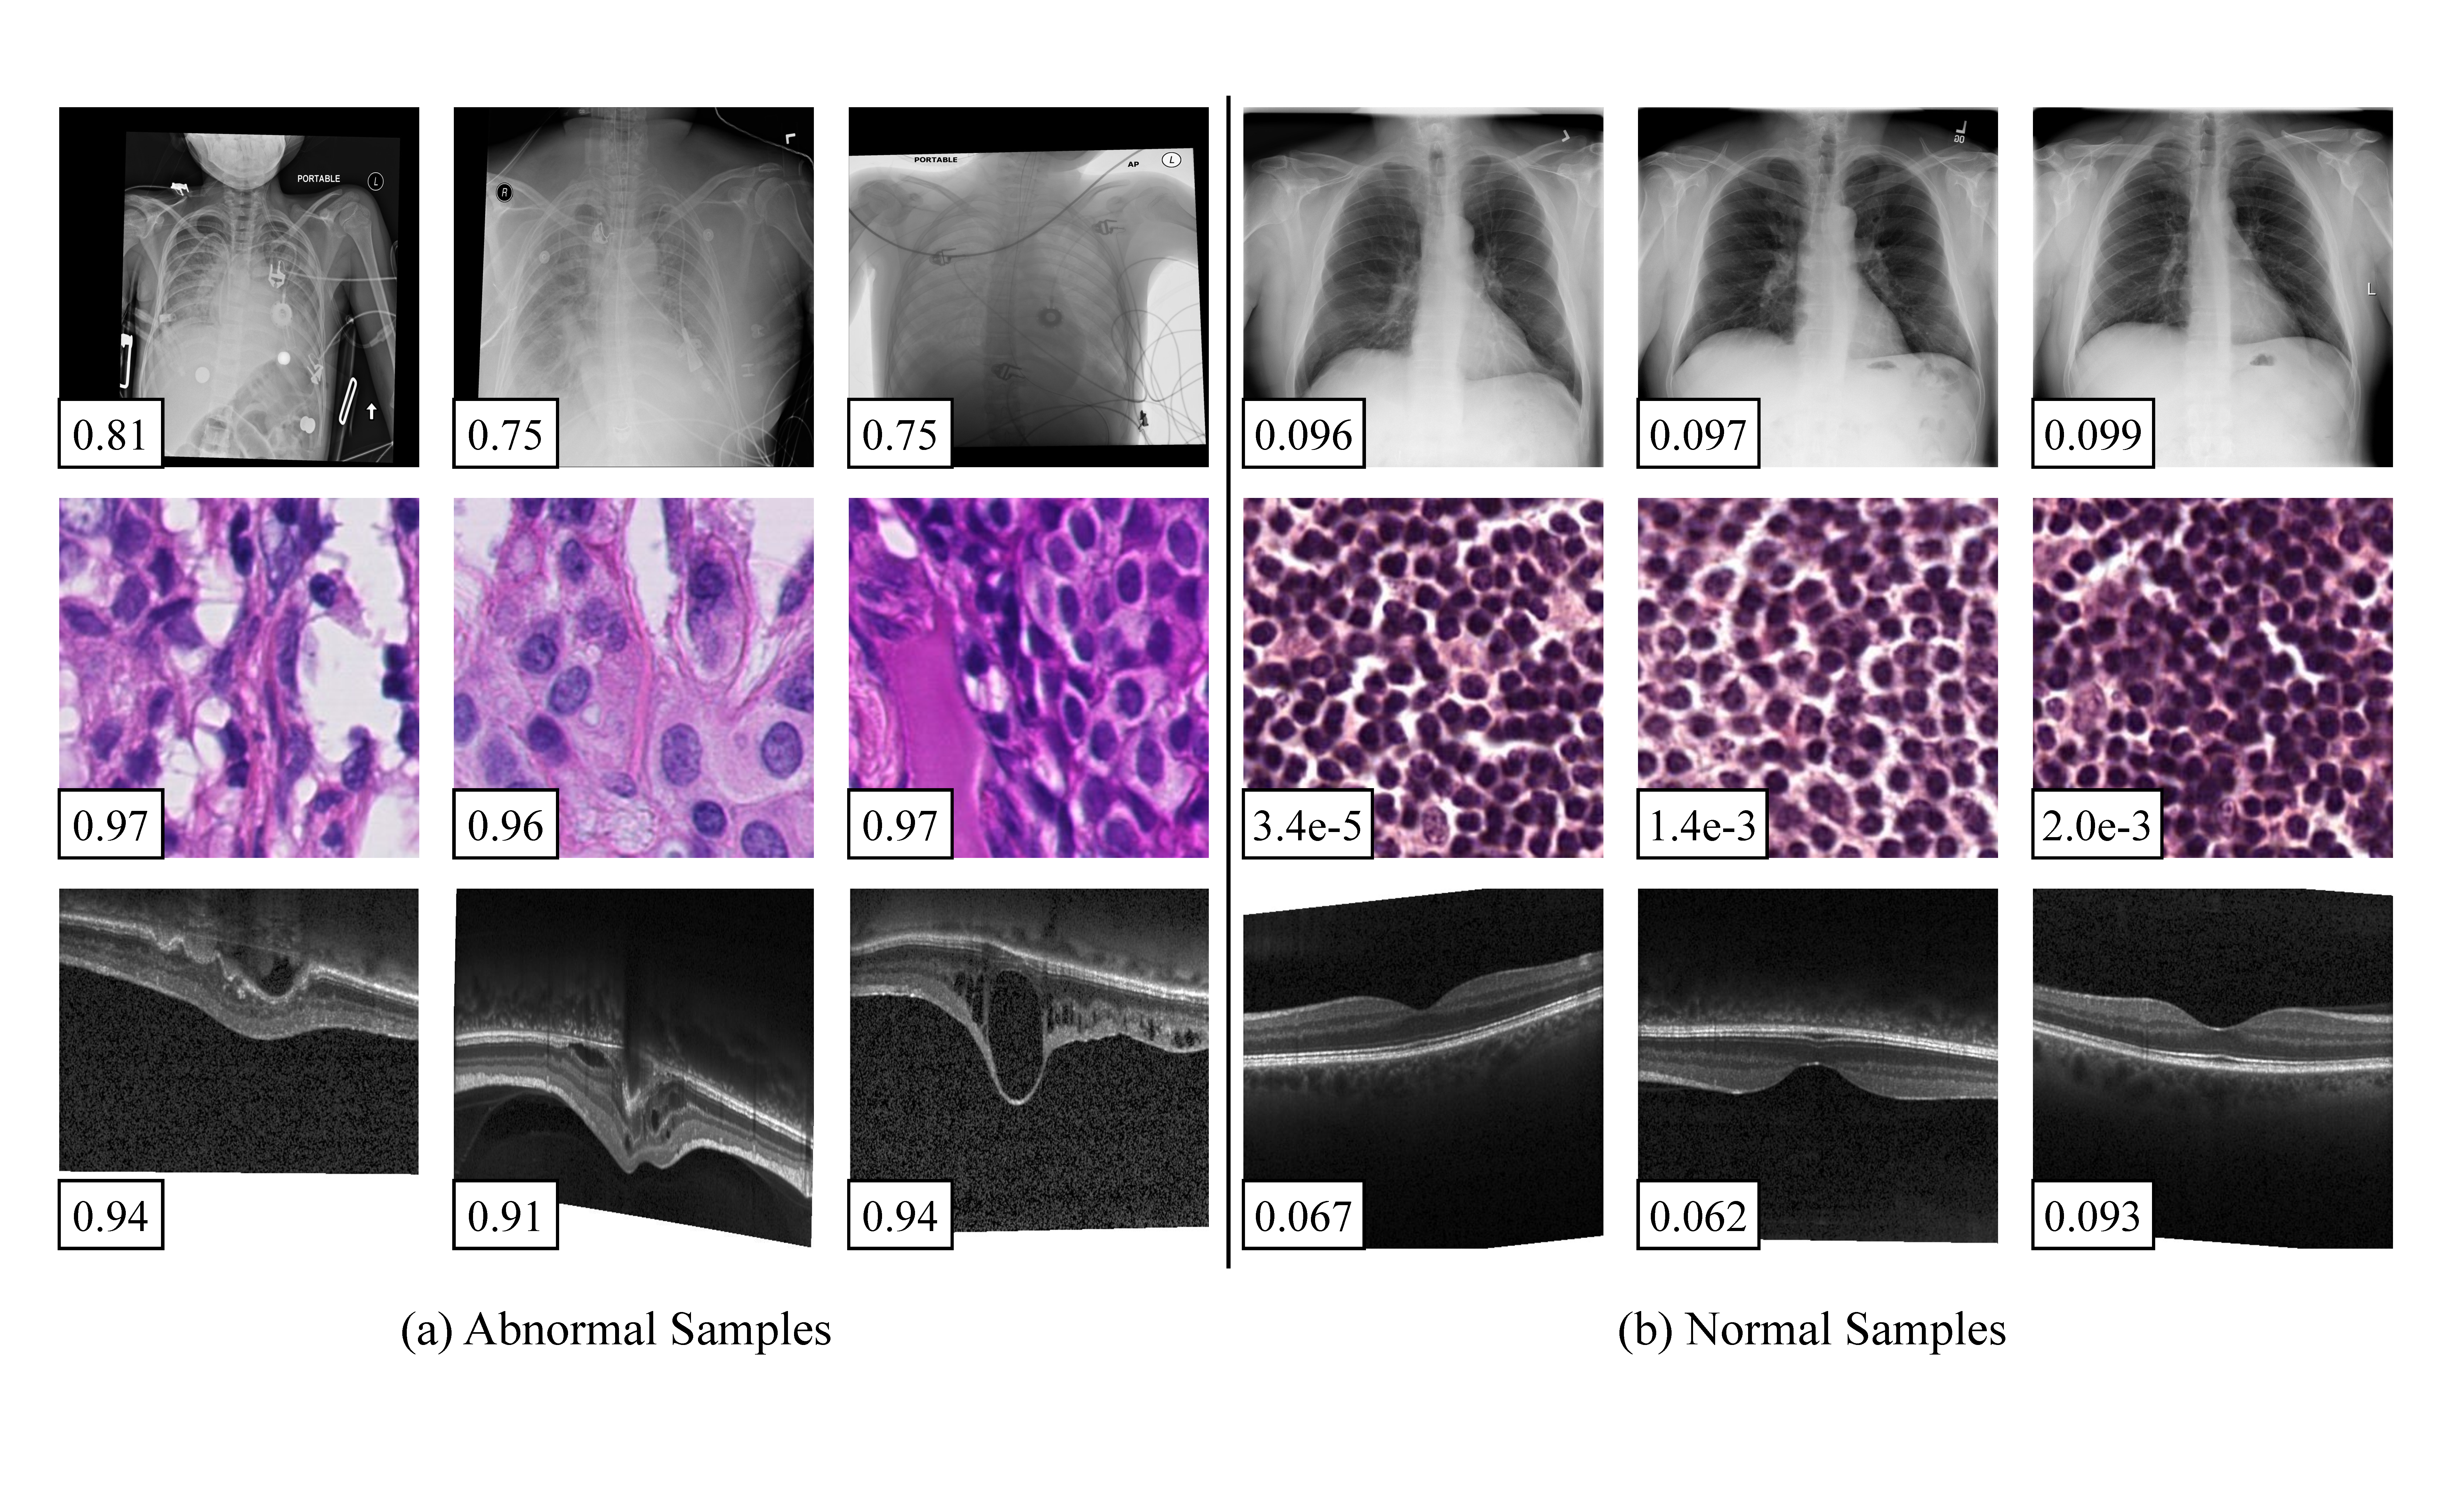
\includegraphics[width=0.6\textwidth]{img/visualize_img_supp.pdf}
    \caption{Examples of (a) abnormal samples and (b) normal samples on chest X-ray, histopathology, and retinal OCT. The predicted scores by our method are shown with each sample. The higher the score, the more likely to be an anomaly.}
    \label{fig:visualimg}
\end{figure*}

\begin{figure*}[h!]
    \centering    
    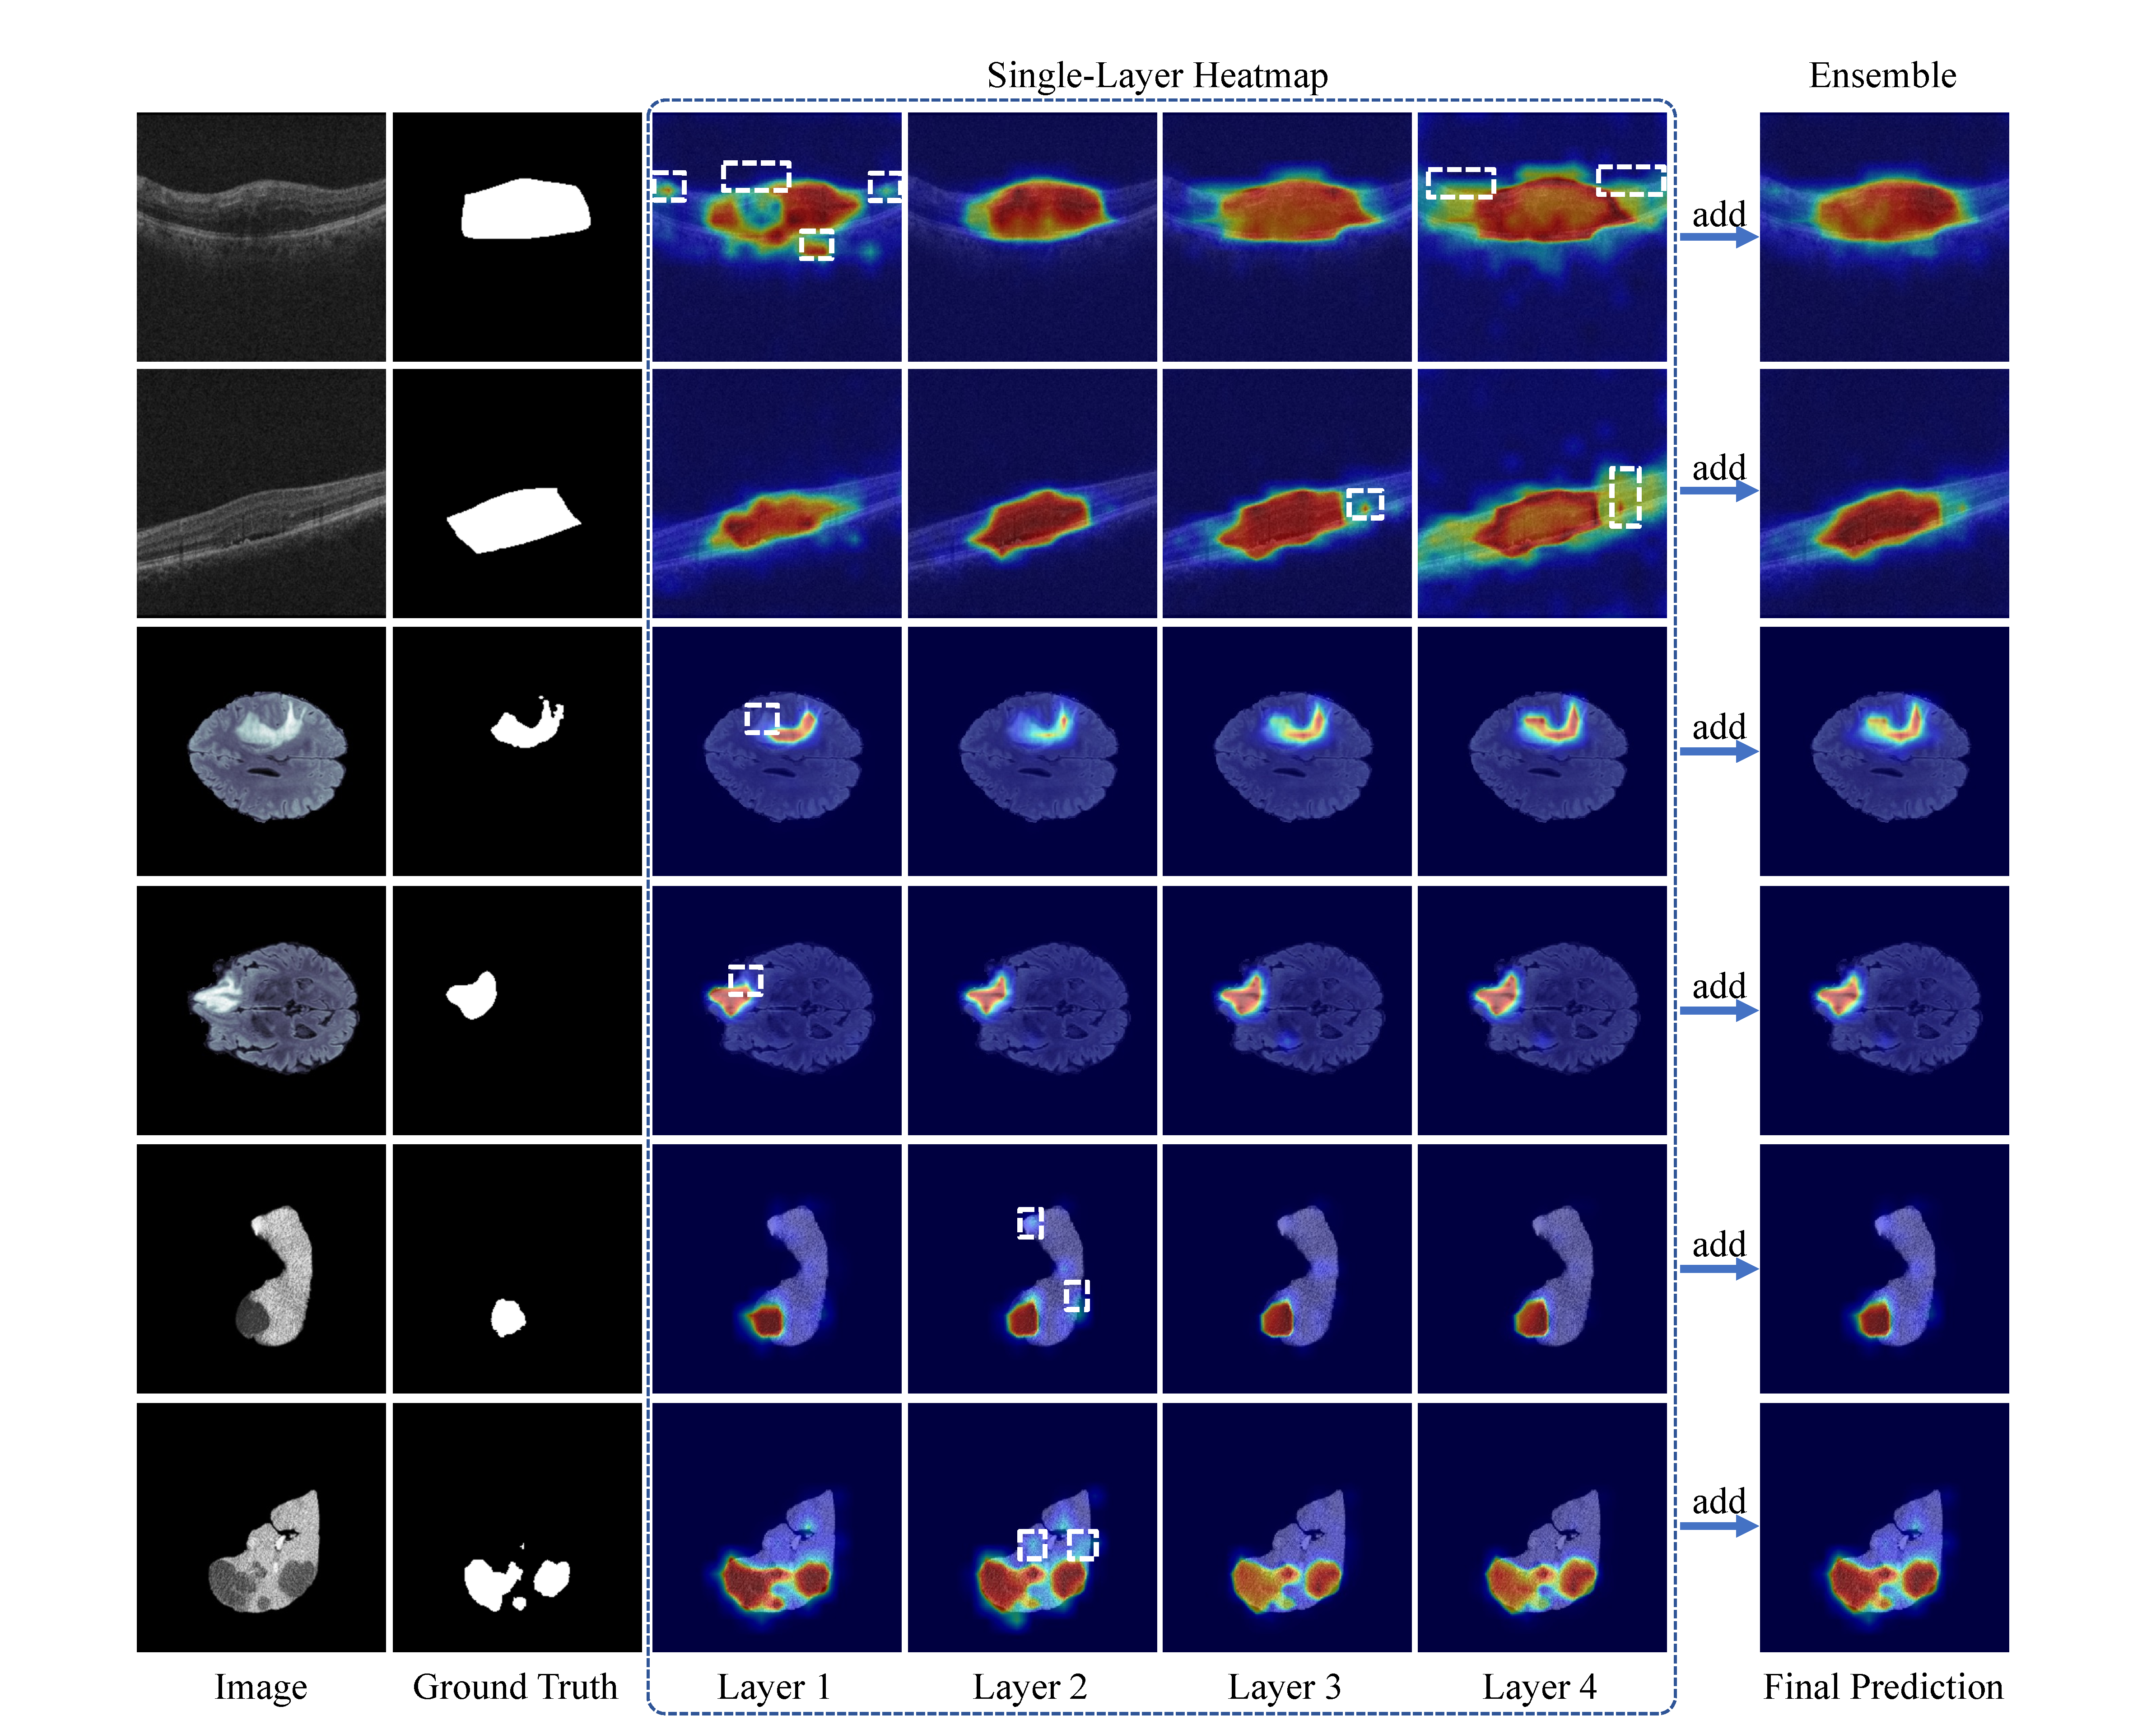
\includegraphics[width=0.75\textwidth]{img/multilayer_supp.pdf}
    \caption{Visualization of anomaly segmentation heatmaps from the four single layers and the multi-layer ensemble results. The white dashed boxes demarcate regions that have been missed or erroneously segmented.}
    \label{fig:multilayer}
\end{figure*}

\begin{figure*}[h!]
    \centering    
    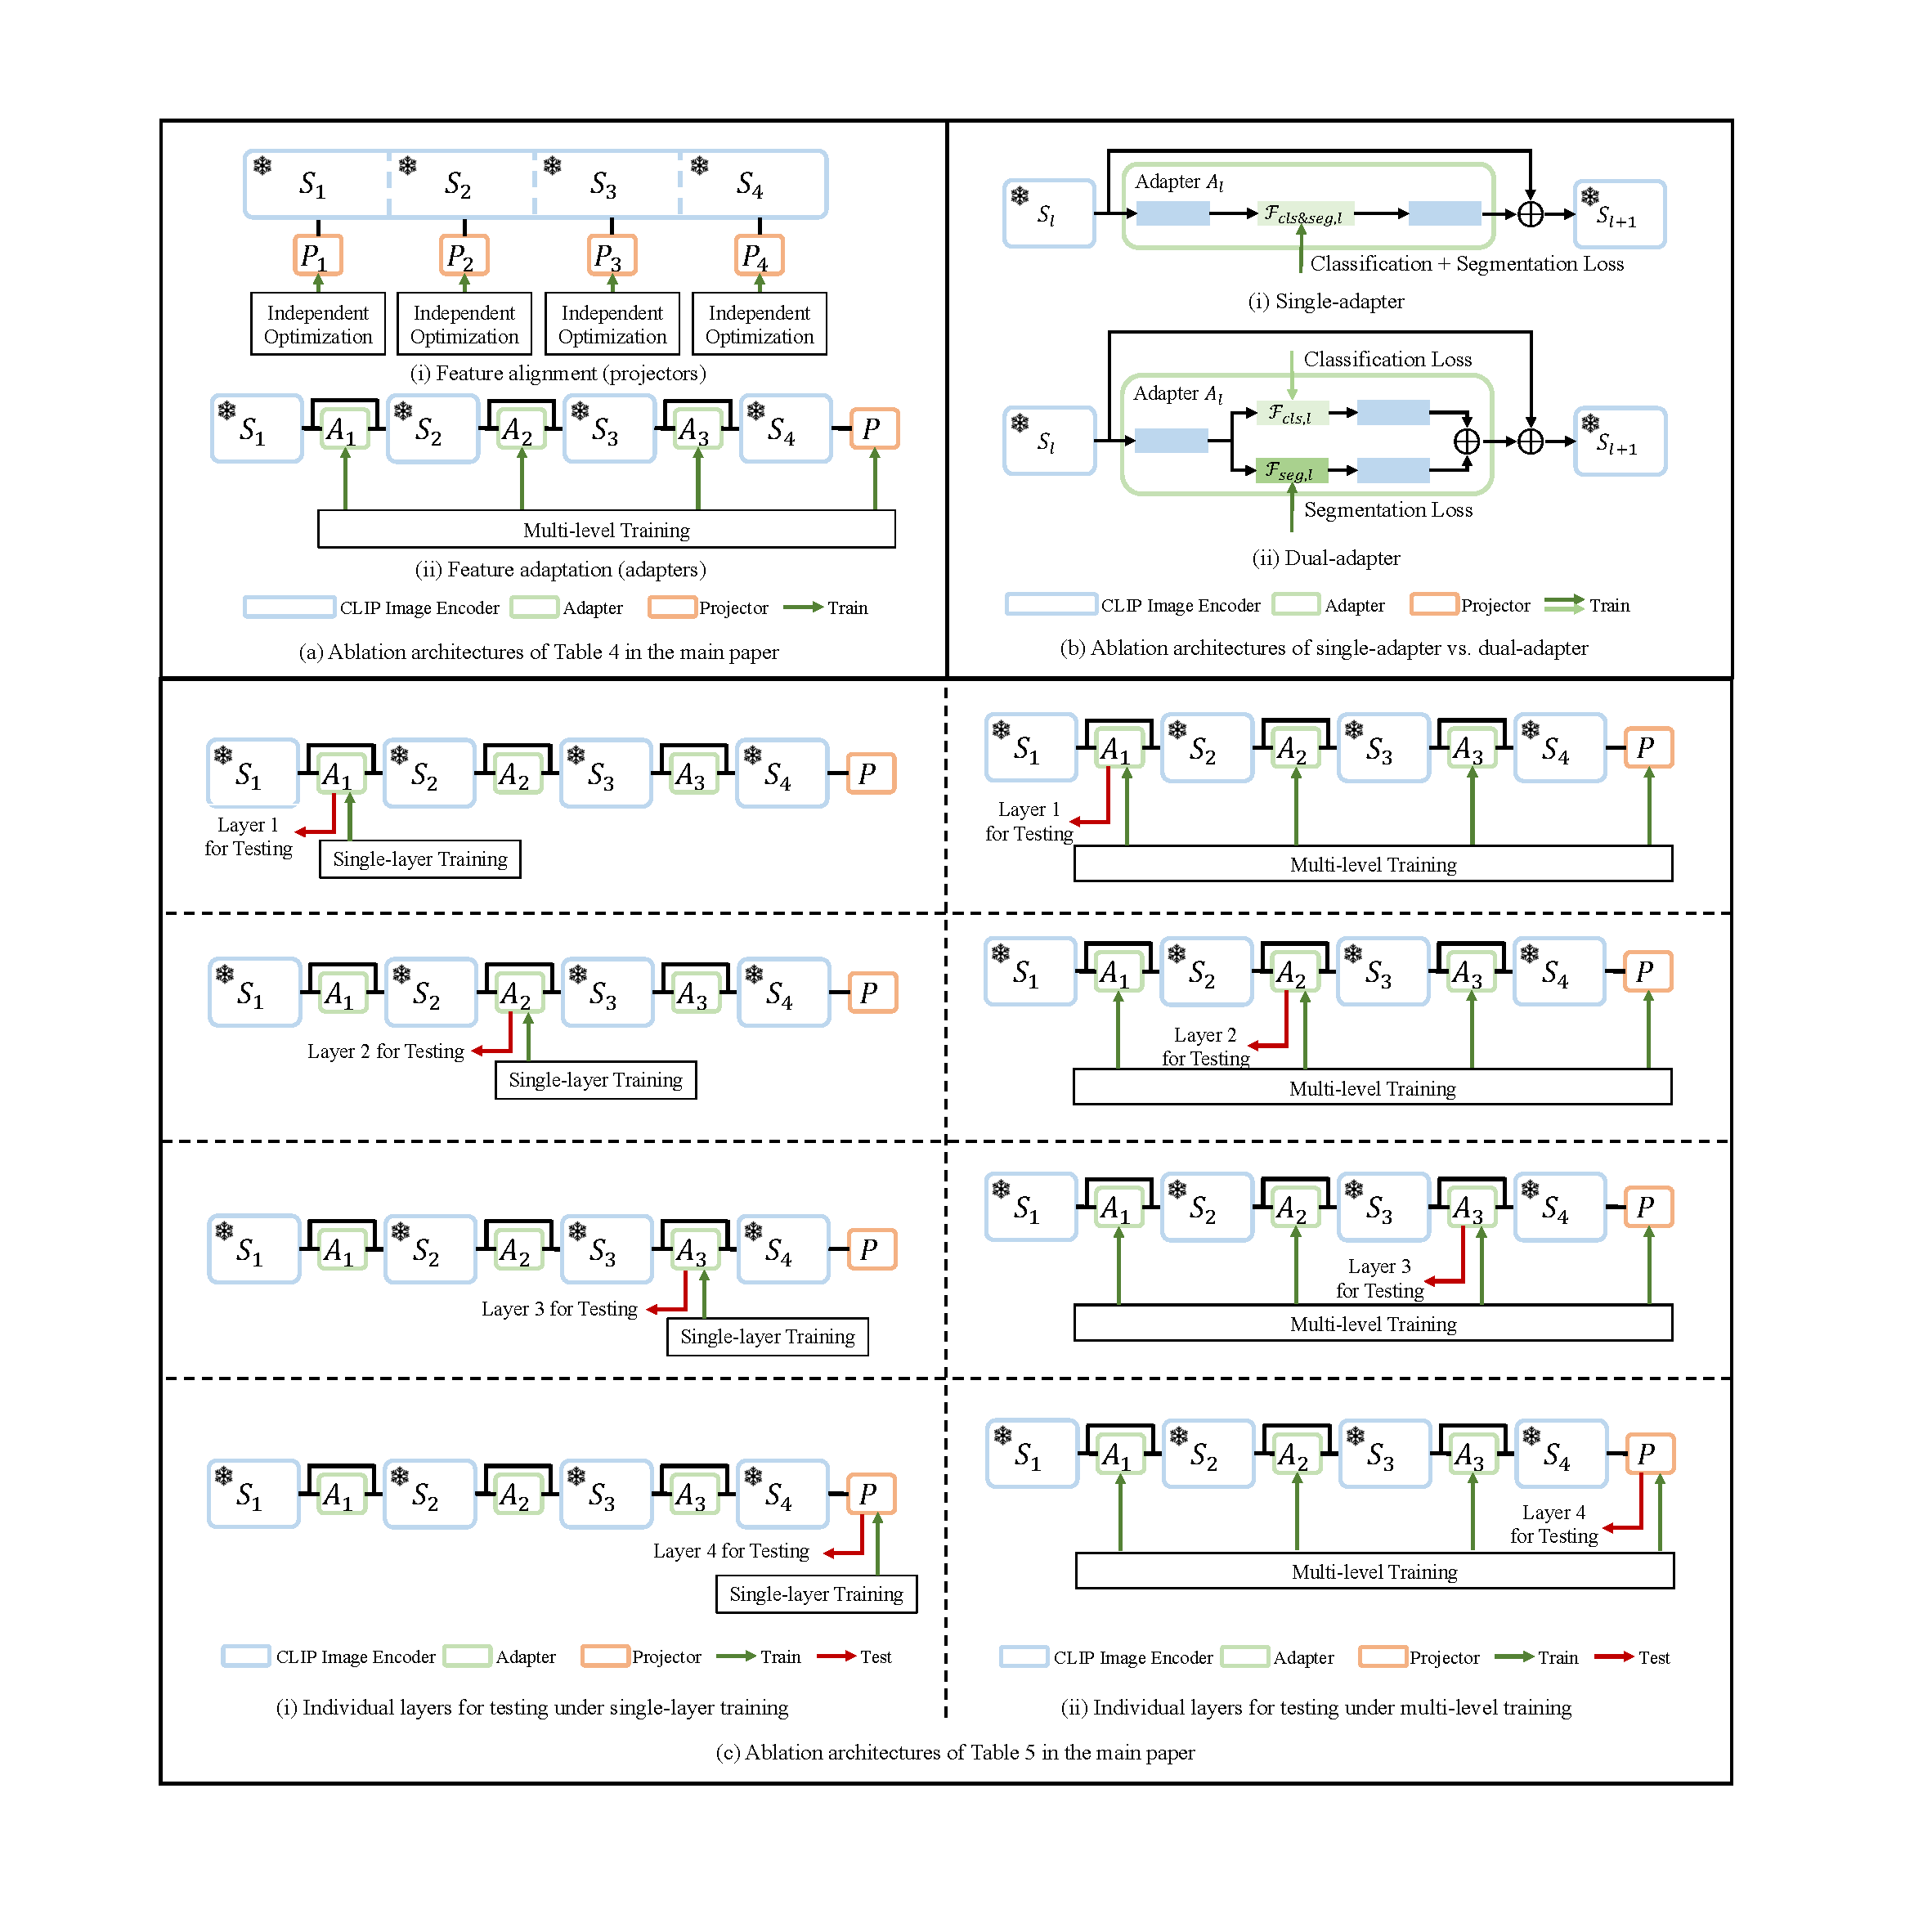
\includegraphics[width=0.75\textwidth]{img/supp.pdf}
    \caption{Model structures corresponding to the ablation experimental settings.}
    \label{fig:abla}
\end{figure*}

\noindent\textbf{BrainMRI:} This dataset is built upon the BraTS2021 dataset~\cite{baid2021rsna,bakas2017advancing,menze2014multimodal}, utilizing 3D FLAIR volumes. To account for variations in brain images at different depths, slices within the depth range of 60 to 100 of the 3D FLAIR volumes are selected. Each extracted 2D slice was saved in PNG format and has an image size of $240\times 240$ pixels. The training set encompasses 7,500 normal samples, while the test set comprises 3,715 samples with a balanced ratio of normal to anomaly instances. 

\noindent\textbf{LiverCT:} Derived from two distinct datasets, BTCV~\cite{landman2015miccai} and LiTS~\cite{bilic2023liver}, this dataset is structured to facilitate anomaly detection. The anomaly-free BTCV set, consisting of 50 abdominal 3D CT scans, constitutes the training set, while the test data comprises 131 abdominal 3D CT scans from LiTS. For both datasets, Hounsfield-Unit (HU) of the 3D scans are transformed into grayscale with an abdominal window. The scans are then cropped into 2D axial slices, containing 1,452 2D slices for training and 1,493 2D slices for testing.

\noindent\textbf{Retinal OCT:} The benchmark includes two different OCT AD datasets. The \textbf{RESC} dataset~\cite{hu2019automated} offers pixel-level segmentation labels, delineating regions affected by retinal edema. In contrast, the \textbf{OCT17} dataset~\cite{kermany2018identifying} primarily serves for classification tasks, featuring retinal OCT images categorized into three types of anomalies.

\noindent\textbf{ChestXray:} This dataset comprises lung images, utilizing RSNA~\cite{wang2017chestx} which was originally provided for a lung pneumonia detection task. Abnormal data encompasses cases of ``Lung Opacity'' and cases of ``No Lung Opacity/Not Normal''. The dataset is partitioned into 8,000 normal training images and 17,194 images for testing.

\noindent\textbf{HIS:} Based on Camelyon16~\cite{bejnordi2017diagnostic}, this dataset encompasses 400 whole-slide images (WSIs) of lymph node sections stained with hematoxylin and eosin (H\&E) from breast cancer patients. The training set incorporates 5,088 randomly extracted normal patches from the original training set. For testing, 1,003 normal and 997 abnormal patches from the 115 testing WSIs are utilized.

\section{Text Prompt Formatting}\label{sec:ap_text}
In this study, we adopt a combination of state-level and template-level prompts for generating textual input for the text encoder, as detailed in Figure~\ref{fig:comp_prompt} and following the approach in~\cite{winclip}. The state-level prompts are ingeniously designed by substituting the token [o] with names of human organs such as ``brain'', ``liver'', etc. This substitution strategy allows us to create a varied range of prompts that can categorize images as ``normal'' or ``abnormal'' based on the organ context. We then incorporate these state-level prompts into broader template-level constructs. By replacing the placeholder [c] in a template-level prompt with a corresponding state-level prompt, we formulate prompts that are both comprehensive and contextually rich. This systematic approach enables the creation of detailed, context-specific prompts that accurately distinguish between the normal and abnormal states.

\section{Additional Quantitative Results}\label{sec:ap_results}
\textbf{Results Varied Shot Numbers:} Table~\ref{tal:suppfew} provides a detailed quantitative analysis on the performance of our medical AD approach, benchmarking it against leading few-shot AD methodologies. This analysis is meticulously tabulated, showing our approach's performance specificity across different shot numbers ($K\in\{2,4,8,16\}$). These results lay the groundwork for a line chart featured in the main paper, which visually captures the subtle differences in performance under various conditions.

\noindent \textbf{Ablation Study on Multi-level Features:} 
We carried out an extensive ablation study to evaluate the effectiveness of utilizing single-layer features for each dataset, in line with the average performances across all datasets discussed in the main paper. The outcomes, elucidated in Table~\ref{tal:supplayer_2}, provide a comprehensive understanding of the performance of single-layer features obtained without the implementation of multi-level training. In contrast, Table~\ref{tal:supplayer} presents the results attained through the strategic implementation of multi-level training techniques.

\noindent \textbf{Evaluation on Industrial Anomaly Detection:} For in-domain evaluation, the MVTec AD benchmark~\cite{bergmann2019mvtec}, consisting of 15 industrial defect detection sub-datasets, is considered. MVFA significantly outperforms competing methods, highlighting its superior generalization capabilities. Detailed results for each sub-dataset are included in Table~\ref{tal:s7_in2}.

\section{Additional Qualitative Results}\label{sec:ap_vis}

\noindent \textbf{Anomaly Classification Instances:} Figure~\ref{fig:visualimg} displays results of AC from datasets that only provide anomaly classification labels. These results were obtained using our method in a few-shot setting (K=4). Each instance is accompanied by a predicted score, ranging from zero to one, where higher scores indicate a higher likelihood of an anomaly.

\noindent \textbf{Ensemble of Multi-level Features:} 
Figure~\ref{fig:multilayer} showcases visualizations from different layers used in the anomaly segmentation task. These visualizations include results from datasets such as BrainMRI, LiverCT, and RESC.

\section{Ablation Model Structure}

To effectively convey the nuances of our ablation study in the main paper, we utilized Figure~\ref{fig:abla} to graphically demonstrate the configurations of the models used in our experiments. Specifically, Figure~\ref{fig:abla} (a) visually details the designs of both the adapter and projector as outlined in Table~\ref{tal:abl1} of the main paper, where part (i) illustrates the projector and part (ii) depicts the adapter. In Figure~\ref{fig:abla} (b), we present the configurations for both the single-adapter and dual-adapter models, shown in subfigures (i) and (ii) respectively. Furthermore, Figure~\ref{fig:abla} (c) illustrates the testing pipeline for assessing the impact of training at different levels. Subfigure (i) represents the scenario of single-layer training, while subfigure (ii) demonstrates the approach for multi-level training, corresponding to the discussions and findings presented in Table~\ref{tal:abl3} of the main paper.

\begin{table}[t]
\centering
\caption{Ablation studies of the architecture of dual-adapter against single-adapter in MVFA. The AUCs (in \%) for classification (AC) and segmentation (AS) under the few-shot setting (K=4) are reported, with the best result marked in bold.}
\label{tal:abl2}
\small
\setlength{\tabcolsep}{1.8pt}{
\begin{tabular}{C{2.0cm}|C{1.4cm}C{1.4cm}C{1.4cm}C{1.4cm}}
\toprule
\multirow{2}{*}{Datasets} & \multicolumn{2}{c}{AC} & \multicolumn{2}{c}{AS}\\
& single-adapter & dual-adapter & single-adapter & dual-adapter\\
\cmidrule(lr){1-5}
HIS & 80.80 & \textbf{82.71} & - & - \\
ChestXray & 78.02 & \textbf{81.95} & - & - \\
OCT17 & \textbf{99.87} & 99.38 & - & - \\
BrainMRI & 92.28 & \textbf{92.44} & 96.98 & \textbf{97.30} \\
LiverCT & 81.07 & \textbf{81.18} & 99.42 & \textbf{99.73} \\
RESC & 94.06 & \textbf{96.18} & 98.53 & \textbf{98.97} \\
\cmidrule(lr){1-5}
average & 87.68 & \textbf{88.97} & 98.31 & \textbf{98.67} \\
\bottomrule
\end{tabular}}
\end{table}

\noindent\textbf{Dual-Adapter vs. Single-Adapter.} We compare the performance of the dual-adapter architecture against the single-adapter setup within the few-shot setting. The dual-adapter design, as implemented in our MVFA model, generates two parallel sets of features at each level, catering to both global (classification) and local (segmentation) aspects. The corresponding architectures are shown in Figure~\ref{fig:abla} (b). According to the results in Table~\ref{tal:abl2}, the dual-adapter approach outperforms the single-adapter model on almost all the datasets. We observed an enhancement in the average AUC for AC, improving from 87.68\% to 88.97\%, and for AS, rising from 98.31\% to 98.67\%. This improvement indicates that the dual-adapter architecture is more effective in managing the demands in medical images.

